\setcounter{chapter}{2} 
\chapter{Theoretical Background: Processes Implemented in the CTM3}\label{Chap:CTM3theory_ocean_hetReact}

Some of the processes that are implemented in the Oslo CTM3 requires some further explanation. This chapter covers the theory behind the implementation of emissions of organic halogen species and the heterogeneous reaction surfaces. These processes are essential to achieve the \acrfull{be} episodes causing the \acrfull{ode}s in the polar tropospheric boundary layer (theory covered in Chapter \ref{ch:theoretical_back}).

\section{Oceanic Emissions of Halocarbons}\label{sec:oceanic_emissions}


The ocean is a natural source of gaseous halocarbons, which are precursors for the reactive \chem{Br}-species that are essential for the bromine explosion to occur (\cite{Schmidt} and references therein)(theory covered in Section \ref{sec:halogen_sources}). Methyl halides ($\chem{CH_3X}$) and polyhalogenated species ($\chem{CHBr_3}$, $\chem{CH_2Br_2}$) are released from the ocean. Methyl halides (particularly $\chem{CH_3Br}$) may also be emitted by biomass burning (\cite{SeinfeldSpyros}). 

\medskip

Natural marine sources of bromoform ($\chem{CHBr_3}$) and dibromomethane ($\chem{CH_2Br_2}$) were used as sources of bromine in this implementation. The component mapping methyl bromide ($\chem{CH_3Br}$) was already included in the Oslo CTM3, which would only be used by the model when the stratosphere was activated \footnote{This was not the case in my runs. The setup is explained in Section \ref{chap:CTM3_Setup}}. In order to further simplify the alterations made in the model, the $\chem{CH_3Br}$-component was used to denote the combined emissions of $\chem{CHBr_3}$ and $\chem{CH_2Br_2}$. As the halogen-induced ODE is the scope of this thesis, it was not considered necessary to implement explicit emissions of these polyhalogenated species, but rather ensure a source of reactive bromine (Equation \ref{R:10}-\ref{R:12}).


\medskip

The anthropogenic signal of methyl halides was not taken into consideration in this thesis. Neither was the difference in lifetime for $\chem{CH_3Br}$ ($94 (84-114)$ days) and $\chem{CHBr_3}$ ($15 (13-7)$ days) (\cite{Hossaini2016_chlorine}) or seasonal variations (\cite{Liang2010}). 


\medskip

Bromoform, $\chem{CHBr_3}$, was added as a source from the ocean based on the emission scenario suggested by \cite{Liang2010} (scenario A, Figure \ref{fig:Liang2010}). This scenario was chosen as it has latitudinal-dependent emission field covering the whole globe. The global emissions estimated by \cite{Liang2010}, scenario A, were 425 Ggyr$^{-1}$ of $\chem{CHBr_3}$ and 57 Ggyr$^{-1}$ of $\chem{CH_2Br_2}$, respectively. $\chem{CH_2Br_2}$ was added to the emission scheme in Figure \ref{fig:Liang2010} by a scaling factor based on the global emissions. The scaling factor is derived below.

\begin{figure}
    \centering
    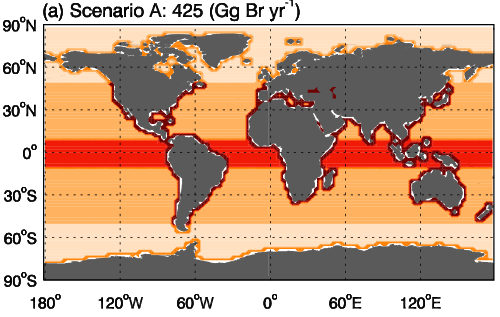
\includegraphics[width = 0.5\textwidth]{Chapter3_Theory_ocean_hetReact/images/liang_etal_2010.png}
    \caption{Global emission distribution of $\chem{CHBr_3}$. Scenario A is applied for the \chem{CHBr_3} with emissions taken as the half point of the colorbar. Image taken from \cite{Liang2010}}
    \label{fig:Liang2010}
\end{figure}
\medskip

The scaling factor was calculated by finding the yield of bromine from both $\chem{CHBr_3}$ and $\chem{CH_2Br_2}$ based on reactions \ref{R:10} and \ref{R:11}, and expressing this in terms of $\chem{CHBr_3}$. 

\begin{align*}
    \chem{X} & = 57 Gg \chem{CH_2Br_2}yr^{-1} \\
    \chem{Y} & = 425 Gg \chem{CHBr_3}yr^{-1} 
\end{align*}

The bromine yield, \chem{Z}, from Reactions \ref{R:10} and \ref{R:11} is then: 

\begin{align*}
    \chem{Z} & = \Big(3\cdot\Big(\frac{X}{M_{\chem{CH_2Br_2}}}\Big) + 2\cdot\Big(\frac{Y}{M_\chem{CHBr_3}}\Big)\Big)\cdot M_{\chem{Br}} \\
    & = \Big(3\cdot\Big(\frac{425 Gg \chem{CHBr_3}yr^{-1}}{252.73 g mol^{-1}}\Big) + 2\cdot\Big(\frac{57 Gg \chem{CH_2Br_2}yr^{-1}}{173.83 g mol^{-1}}\Big)\Big)\cdot79.90 g mol^{-1} \\
    & = 455 Gg\chem{Br}yr^{-1}
\end{align*}

The emission of $\chem{CHBr_3}$, had this been the only source of bromine, is expressed by $Y'$, which is: 

\begin{align*}
    \chem{Y'} & = \frac{1}{3}\cdot\frac{252.73 g mol^{-1}}{79.90 g mol^{-1}}\cdot455.49Gg\chem{Br}yr^{-1} \\
    & = 479.73 Gg \chem{CHBr_3}yr^{-1}
\end{align*}

This is used in the scaling factor, $f$:

\begin{equation*}
    f = \frac{\chem{Y'}}{Y} \approx 1.13
\end{equation*}


Emissions are then found according to their latitudinal band, and whether the grid box is located over ocean or the coast (for more information about the actual implementation, see Section \ref{sec:tropchem_oslo}). If the location is above 50 $^o$ North over ocean, for example, the emission is taken to be $0.05\times10^{-13}$ kgm$^{-2}$s$^{-1}\times f$. (The conversion to molecules cm$^{-3}$s$^{-1}$ can be seen in Section \ref{sec:tropchem_oslo}). 


\subsection{Emission Inventory}

The emission inventory of $\chem{CHBr_3}$ and $\chem{CH_2Br_2}$ by \cite{Liang2010} was compared against observations and other emission inventories by \cite{Hossaini2013}. The results can be seen in Figures \ref{fig:Hosaini_fig5} and \ref{fig:Hosaini_fig6} in the Appendix. They show a reasonable agreement between the observations and mixing ratios suggested by \cite{Liang2010} for the stations \acrfull{alt}, \acrfull{brw} and Summit (SUM), which are of most relevance in this case. The inventory, however, is rather simplified as it does not take into account seasonality and agreement with observations outside the polar regions. 



\section{Chemical Kinetics and Photoprocesses}\label{sec:chem_kinetics}

This section contains a description of the rate expressions for bimolecular and 3-body reactions as well as photolysis reactions. The reaction rate constants for the bimolecular and 3-body reactions implemented in the troposphere can be seen in Table \ref{tab:2b_and_3b_reactions}, and the photochemical reactions are listed in Table \ref{tab:photolysis_reactions}.

\begin{table}[ht]
\centering
\resizebox{14cm}{!}{%
\begin{tabular}{|c|ccc|c|c|c|l|}
\hline
\multicolumn{8}{|c|}{\textbf{Reactions dependent on temperature (Bimolecular reactions)}}                                                                                                                                                                                                                                                                                                         \\ \hline
\textbf{Reaction}                                                    & \multicolumn{1}{c|}{\textbf{A-factor}}    & \multicolumn{2}{c|}{\textbf{E/R}}                                            & \textbf{k (273.15 K) (*)}                          & \multicolumn{3}{l|}{\textbf{Reaction ref.}}                                                                            \\ \hline
$\chem{Cl} + \chem{CH_4} \rightarrow \chem{HCl} + \chem{CH_3} $      & \multicolumn{1}{c|}{$7.3\cdot10^{-12}$}   & \multicolumn{2}{c|}{$1280$}                                                  & $6.7\cdot10^{-14}$                             & \multicolumn{3}{c|}{\ref{R:cl_ch4}}                                                                                    \\
$\chem{O_3} + \chem{Br} \rightarrow \chem{BrO} + \chem{O_2}$         & \multicolumn{1}{c|}{$1.7\cdot10^{-11}$}   & \multicolumn{2}{c|}{$800$}                                                   & $9.1\cdot10^{-13}$                             & \multicolumn{3}{c|}{\ref{R:2}}                                                                                         \\
$\chem{O_3} + \chem{Cl} \rightarrow \chem{ClO} + \chem{O_2}$         & \multicolumn{1}{c|}{$2.3\cdot10^{-11}$}   & \multicolumn{2}{c|}{$200$}                                                   & $1.1\cdot10^{-11}$                             & \multicolumn{3}{c|}{\ref{R:2}}                                                                                         \\
$\chem{BrO} + \chem{BrO} \rightarrow 2\chem{Br} + \chem{O_2}$        & \multicolumn{1}{c|}{$2.4\cdot10^{-12}$}   & \multicolumn{2}{c|}{$-40$}                                                   & $2.8\cdot10^{-12}$                             & \multicolumn{3}{c|}{\ref{R:4}}                                                                                         \\
$\chem{OH} + \chem{ClO} \rightarrow \chem{Cl} + \chem{HO_2}$         & \multicolumn{1}{c|}{$7.4\cdot10^{-12}$}   & \multicolumn{2}{c|}{$-270$}                                                  & $2.0\cdot10^{-11}$                             & \multicolumn{3}{c|}{\ref{R:15}}                                                                                        \\
$\chem{BrO} + \chem{HO_2} \rightarrow \chem{HOBr} + \chem{O_2}$      & \multicolumn{1}{c|}{$4.5\cdot10^{-12}$}   & \multicolumn{2}{c|}{$-460$}                                                  & $2.4\cdot10^{-11}$                             & \multicolumn{3}{c|}{\ref{R:6}}                                                                                         \\
$\chem{Br} + \chem{HO_2} \rightarrow \chem{HBr} + \chem{O_2}$        & \multicolumn{1}{c|}{$4.8\cdot10^{-12}$}   & \multicolumn{2}{c|}{$310$}                                                   & $1.5\cdot10^{-12}$                             & \multicolumn{3}{c|}{\ref{R:17}}                                                                                        \\
$\chem{OH} + \chem{ClO} \rightarrow \chem{HCl} + \chem{O_2}$         & \multicolumn{1}{c|}{$6.0\cdot10^{-13}$}   & \multicolumn{2}{c|}{$-230$}                                                  & $1.4\cdot10^{-12}$                             & \multicolumn{3}{c|}{\ref{R:16}}                                                                                        \\
$\chem{BrO} + \chem{NO} \rightarrow \chem{NO_2} + \chem{Br}$         & \multicolumn{1}{c|}{$8.8\cdot10^{-12}$}   & \multicolumn{2}{c|}{$-260$}                                                  & $2.3\cdot10^{-11}$                             & \multicolumn{3}{c|}{\ref{R:14}}                                                                                        \\
$\chem{CHBr_3} + \chem{OH} \rightarrow 3\chem{Br} + \chem{Products}$ & \multicolumn{1}{c|}{$1.35\cdot10^{-12}$}  & \multicolumn{2}{c|}{$600$}                                                   & $1.5\cdot10^{-13}$                             & \multicolumn{3}{c|}{\ref{R:10}}                                                                                        \\ \hline
\multicolumn{8}{|c|}{\textbf{Reactions dependent on pressure and temperature (3-body reactions)}}                                                                                                                                                                                                                                                                         \\ \hline
\multirow{2}{*}{\textbf{Reaction}}                                   & \multicolumn{3}{c}{\textbf{Low-Pressure Limit}}                                                                          & \multicolumn{3}{c|}{\textbf{High-Pressure Limit}}                                                                             & \multirow{2}{*}{\textbf{Reaction ref.}} \\ \cline{2-7}
                                                                     & \multicolumn{1}{c|}{\textbf{k$_0^{300}$}} & \multicolumn{1}{l|}{\textbf{n}} & \multicolumn{1}{l|}{\textbf{k$_0^{300}$ (273.15 K) (**)}} & \multicolumn{1}{l|}{\textbf{k$_\infty^{300}$}} & \multicolumn{1}{l|}{\textbf{m}} & \multicolumn{1}{l|}{\textbf{k$_\infty^{300}$ (273.15 K) (***)}} &                                         \\ \hline
$\chem{BrO} + \chem{NO_2} + M \rightarrow \chem{BrONO_2} + M$        & \multicolumn{1}{c|}{$5.2\cdot10^{-31}$}   & \multicolumn{1}{c|}{$3.2$}      & $7.0\cdot10^{-31}$                         & $6.9\cdot10^{-12}$                             & $2.9$                           & $9.0\cdot10^{-12}$                         & \multicolumn{1}{c|}{\ref{R:9}}          \\
$\chem{NO_2} + \chem{ClO} + M \rightarrow \chem{ClONO_2} + M $       & \multicolumn{1}{c|}{$1.8\cdot10^{-31}$}   & \multicolumn{1}{c|}{$3.4$}      & $2.5\cdot10^{-31}$                         & $1.5\cdot10^{-11}$                             & $1.9$                           & $1.8\cdot10^{-11}$                         & \multicolumn{1}{c|}{\ref{R:clono2}}     \\ \hline
\end{tabular}
}
\caption{Rate coefficients for some of the bimolecular and 3-body reactions implemented in the troposphere. Values are taken from \cite{JPL}. Rate coefficients are calculated at 273.15 K by: 
\\ 
(*) k is calculated by Equation \ref{eq:2b_rate_coeff} 
\\ 
(**) k$_0^{300}$ is calculated by Equation \ref{eq:3b_low_pressure} 
\\ 
(***) k$_\infty^{300}$ is calculated by Equation \ref{eq:3b_high_pressure}} 
\label{tab:2b_and_3b_reactions}
\end{table}

\begin{table}[]
\centering
\begin{tabular}{|l|l|}
\hline
\textbf{Reaction}                                             & \textbf{Reaction ref.} \\ \hline
$\chem{BrCl} + hv \rightarrow \chem{Br} + \chem{Cl}$          & \ref{R:19}             \\
$\chem{Br_2} + hv \rightarrow 2\chem{Br}$                     & \ref{R:1}              \\
$\chem{BrO} + hv \rightarrow \chem{Br} + \chem{O}$                & \ref{R:20}             \\
$\chem{HOBr} + hv \rightarrow \chem{OH} + \chem{Br}$          & \ref{R:18}             \\
$\chem{CHBr_3} + hv \rightarrow 3\chem{Br} + \text{Products}$ & \ref{R:12}             \\ \hline
\end{tabular}
\caption{Photolysis reactions added in the troposphere}
\label{tab:photolysis_reactions}
\end{table}


\subsection{Bimolecular Reactions}\label{sec:bimolecular_reactions}

Bimolecular reactions are reactions in which two chemical species react and produce a different set of species (\cite{Jacob1999}). A bimolecular (two-body) reaction can be written as: 

\begin{equation*}
    A + B \rightarrow C + D
\end{equation*}

%A direct bimolecular reaction is a reaction in which \chem{A} and \chem{B} goes on to produce \chem{C} and \chem{D} without an intermediate formation of an \chem{AB}-bond, but rather has a transition state $(\chem{AB})^\neq$ that lies between the reactants and products (\cite{JPL}). 

%\medskip

%The correlation between the expected structure of $(\chem{AB})^\neq$ and the A-factor (Arrhenius factor) of the the reaction rate constant


The reaction rate, $k$, is the time rate of change of a concentration of the reactant in the reaction (\cite{AtmModFund}). It is given by: 

\begin{equation*}
    -\frac{d}{dt}[A] = -\frac{d}{dt}[B] = \frac{d}{dt}[C] = \frac{d}{dt}[D] = k[A][B]
\end{equation*}

in which the bracketed species $[]$ denotes the number densities (in this case the number of molecules per $cm^3$) and $k$ is the second-order rate coefficient for the reaction in $cm^3\text{molecule}^{-1}s^{-1}$. The product $[A][B]$ is proportional to the frequency of collisions. A bimolecular reaction could also be a self-reaction, in which $B = A$ and the reaction rate would be:

\begin{equation*}
    -\frac{d}{dt}[A] = -\frac{d}{dt}[A] = \frac{d}{dt}[C] = \frac{d}{dt}[D] = k[A]^2
\end{equation*}

The rate coefficients are given in Table \ref{tab:2b_and_3b_reactions} in Arrhenius form (for more information, see \cite{JPL}):

\begin{equation}
    k(T) = A\cdot\exp{\Big(-\frac{E/R}{T}\Big)}
    \label{eq:2b_rate_coeff}
\end{equation}

In which $A$ is the Arrhenius-factor, $E/R$ is the temperature dependence (activation temperature) and $T$ is the temperature. 

\subsection{3-Body Reactions}\label{sec:3body_reactions}

Three-body reactions are reactions in which two chemical species, \chem{A} and \chem{B}, react to produce one single product species, \chem{AB}, helped by a third body, $M$ (\cite{Jacob1999}). A three-body reaction can be written as: 

\begin{equation*}
    \chem{A} + \chem{B} + M \rightarrow \chem{AB} + M
\end{equation*}


The third body, $M$, is an inert molecule (generally $\chem{N_2}$ or $\chem{O_2}$ in the atmosphere) that removes excess energy from the excited species $\chem{AB*}$ leaving the product species \chem{AB} in its unexcited state (\cite{Jacob1999}).


\medskip

%The rate coefficient for a 3-body reaction is defined as the formation rate of AB by the reaction of $M$ with the excited complex $[\chem{AB}^*]$: 

%\begin{equation*}
%    \frac{d[\chem{AB}]}{dt} = k_3[\chem{AB}^*][M]
%\end{equation*}

%This rate is assumed to be in steady state at all times as $[\chem{AB}^*]$ is very short lived, which leads to the following expression: 

%\begin{equation*}
%    k_1[\chem{A}][\chem{B}] = k_2[\chem{AB}^*] + %k_3[\chem{AB}^*][M]
%\end{equation*}

The rate coefficients for 3-body reactions can be pressure dependent, and therefore have a low-pressure and high-pressure limit. The low pressure limiting rate constants are given in Table \ref{tab:2b_and_3b_reactions} on the form: 

\begin{equation}
    k_0(T) = k_0^{300}\Big(\frac{T}{300}\Big)^{-n}    
    \label{eq:3b_low_pressure}
\end{equation}

In which $k_0^{300}$ is an estimate of the low-pressure limiting rate constant at 300 K and $n$ is the estimated temperature dependence at the low-pressure limit (for more information, see \cite{JPL}). The low pressure rate constants is of third order and has units $cm^6\text{molecule}^{-1}s^{-1}$ (\cite{AtmModFund}).

\medskip

Similarly, there exists a high-pressure limit:

\begin{equation}
    k_\infty(T) = k_\infty^{300}\Big(\frac{T}{300}\Big)^{-m}
    \label{eq:3b_high_pressure}
\end{equation}

In which $k_\infty^{300}$ is an estimate of the high-pressure limiting rate constant at 300 K and $m$ is the estimated temperature dependence at the high-pressure limit (for more information, see \cite{JPL}). The high-pressure rate constant is of second order and has units $cm^3\text{molecule}^{-1}s^{-1}$ (\cite{AtmModFund}).


\subsection{Photochemical Reactions}\label{sec:pchem_reactions}

Photochemical reactions are unimolecular (one-body), i.e. a molecule is hit by a single photon of radiation and breaks into two or more products (\cite{AtmModFund}):

\begin{equation*}
    A + hv \rightarrow B + C
\end{equation*}

The loss rate of \chem{A} is: 

\begin{equation*}
    \frac{d[A]}{dt} = -J[A]
\end{equation*}

In which $J$ is the first-order photolysis rate coefficient of \chem{A} in $s^{-1}$. 


\section{Heterogeneous Chemistry}\label{sec:het_chem}

Heterogeneous reactions occur when a reactant in the gas phase diffuses on the surface of a particle (\cite{DAVIES2018}). This section contains the theory behind the implementation of heterogeneous reactions at aerosol surfaces (Section \ref{sec:aerosol_react}) and over snow/ice surfaces (Section \ref{sec:snow_ice_react}). The heterogeneous reactions that were implemented can be seen in Table \ref{tab:het_reactions}. 

\begin{table}[h]
\centering
\begin{tabular}{|l|l|}
\hline
\textbf{Reaction}                                                                         & \textbf{Reaction ref.} \\ \hline
$\chem{BrONO_2} + \chem{H_2O} \xrightarrow{aerosol} \chem{HOBr} + \chem{HNO_3}$           & \ref{R:13}             \\
$\chem{HOBr} + \chem{H^+} + \chem{Br^-} \xrightarrow{snow/ice} \chem{Br_2} +\chem{H_2O} $ & \ref{R:7}              \\
$\chem{HOBr} + \chem{H^+} + \chem{Cl^-} \xrightarrow{snow/ice} \chem{BrCl} +\chem{H_2O} $ & \ref{R:7}              \\
$\chem{HOBr} + \chem{HCl} \xrightarrow{aerosol} \chem{BrCl} + \chem{H_2O}$                & \ref{R:8}              \\
$\chem{HOBr} + \chem{HBr} \xrightarrow{aerosol} \chem{Br_2} + \chem{H_2O}$                & \ref{R:8}              \\ \hline
\end{tabular}
\caption{Heterogeneous reactions added in the troposphere}
\label{tab:het_reactions}
\end{table}

\subsection{Heterogeneous Reactions on Aerosol Surfaces (Reactions \ref{R:8} and \ref{R:13})}\label{sec:aerosol_react}

The implementation of the heterogeneous aerosol Reactions \ref{R:13} and \ref{R:8} is based on the method described by \cite{CAO}. An overview of the constants used can be found in Table \ref{tab:constants}.

\medskip

The explanation for Reaction \ref{R:8} will be for $\chem{X} = \chem{Br}$, but the same applies to $\chem{X} = \chem{Cl}$. Reaction \ref{R:13} is differently treated ($\gamma$ is parameterized), and is explained further in Section \ref{sec:het_aerosol_react_CTM3}. The production rate of $\chem{Br_2}$ molecules for Reaction \ref{R:8} is (\cite{schwartz1986}): 

\begin{equation*}
    \frac{d}{dt}[\chem{Br_2}] = -\frac{d}{dt}[\chem{HOBr}] = k[\chem{HOBr}]
\end{equation*}

which has a first-order reaction-rate constant dependent on the concentration of \chem{HBr}: 

\begin{equation}
    k = \big(\frac{a}{D_g} + \frac{4}{v_{therm}\gamma}\big)^{-1}\alpha_{eff}
    \label{eq:reaction_rate_const}
\end{equation}

$a$ is a typical aerosol radius (taken as $a = 0.45 \mu m$), $D_g$ is the molecular diffusivity in the gas-phase (taken as $D_g = 0.2  cm^2s^{-1}$), and the ratio $a/D_g$ represents the molecular diffusion limit (\cite{CAO}). 

\medskip

$v_{therm}$ in Equation \ref{eq:reaction_rate_const} is the mean molecular speed of \chem{HOBr} as the impinging gas on the aerosol surface. This is given as:

\begin{equation*}
    v_{therm} = \sqrt{\frac{8RT}{\pi \chem{M_{HOBr}}}}
\end{equation*}

in which $R$ is the universal gas constant (in $Latm/Kmol$), $T$ is the absolute temperature in Kelvin,  and $\chem{M_{HOBr}}$ is the molas mass of \chem{HOBr}. $v_{therm}$ has units $cm/s$. 

\medskip

Finally, the two remaining parameters of Equation \ref{eq:reaction_rate_const} are $\gamma$ and $\alpha_{eff}$. $\gamma$ is the uptake coefficient or reaction efficiency of \chem{HOBr} on sea salt aerosols, i.e. the probability that the reaction will occur (\cite{SeinfeldSpyros}). $\alpha_{eff}$ is the surface-volume coefficient, i.e. the ratio of the total aerosol surface area, $A_{\text{aerosol}}$, and the total volume, $V$ and has the units $[cm^2cm^{-3}]$.
 
\medskip

The production rate of $\chem{Br_2}$ in Reaction \ref{R:8} is limited by the absorption of \chem{HOBr} and \chem{HBr} in the suspended aerosol particles (\cite{CAO}). The probability of the reaction, i.e. the uptake coefficient for \chem{HOBr}, $\gamma$,  can be expressed as (\cite{Hanson1994}) (Values are listed in Table \ref{tab:constants}): 

\begin{equation}
    \frac{1}{\gamma} = \frac{1}{\alpha}+ \frac{v_{therm}}{4H^*RT\sqrt{k_{liq}^ID_{liq}}f(q)}
    \label{eq:upt_coeff}
\end{equation}

in which $\alpha$ is the mass accommodation coefficient. This quantity describes the probability that a gas or vapour particle will stick upon collision with the surface of a particle, where $0\leq\alpha\leq1$ (\cite{SeinfeldSpyros}). Following \cite{CAO}, this will be taken as unity. As before, $R$ is the universal gas constant and $T$ is the temperature. $D_{liq}$ is the liquid phase diffusion coefficient which is a proportionality factor implying that a mass of the substance diffuses through a unit surface in a unit time at a concentration gradient of unity. $H^*$ is the effective Henry's law constant for \chem{HBr}. The Henry's law coefficient, $H$, is a proportionality factor between the amount of dissolved gas and it's partial pressure in the gas phase (\cite{Sander2015}, see also Section \ref{sec:wet_dep_henrys_law}). $k_{liq}^I$ is the first-order liquid reaction rate constant for \chem{HBr}, calculated by: 

\begin{equation}
    k_{liq}^I = k_{liq}^{II}[\chem{HBr}]_{liq}= k_{liq}^{II}H^*_\chem{HBr}P_\chem{HBr}
\end{equation}

In which $H^*_\chem{HBr}$ is the effective Henry's law constant for the species. $P_\chem{HBr}$ is it's partial pressure given by:

\begin{equation*}
    P_\chem{HBr} = \frac{\chem{M_{HBr}}RT}{Av}
\end{equation*}

which is where the dependence of the concentration of \chem{HBr} (in molecules$cm^{-3}$) appears, by $\chem{M_{HBr}}$. $R$ is the universal gas constant (converted from $LatmK^{-1}mol^{-1}$ to $10^3cm^3K^{-1}mol^{-1}$). $T$ is the temperature in Kelvin, and $Av$ is Avogadros number. 

\medskip

Lastly, $f(q)$ in Equation \ref{eq:upt_coeff} is determined by: 

\begin{equation}
    f(q) = \coth{q} -\frac{1}{q} = \frac{1}{\tanh{q}} -\frac{1}{q}
\end{equation}

where $q = a\sqrt{\frac{k_{liq}^I}{D_{liq}}}$ is a dimensionless quantity called the diffuso-reactive parameter. This is used to calculate the uptake rates (\cite{Hanson1994}). 


\subsection{Heterogeneous Reactions Over Snow and Ice Surfaces (Reactions \ref{R:7})}\label{sec:snow_ice_react}


As for the heterogeneous aerosol reactions, the implementation of the heterogeneous reactions over snow/ice surfaces also follows the method by \cite{CAO}. 

\medskip

The rate of change in concentration for Reactions \ref{R:7} can be given as: 

\begin{equation*}
    -\frac{d}{dt}[\chem{HOBr}] = k[\chem{HOBr}]
\end{equation*}

in which the deposition-rate constant, $k$, is: 

\begin{equation*}
    k = \frac{v_d}{L_{mix}}\beta
\end{equation*}

Thus, the deposition-rate constant depends on the deposition velocity, $v_d$, at the snow/ice surface, the height of the boundary layer, $L_{mix}$ and the reactive surface ratio coefficient, $\beta$. 

\medskip

The deposition velocity, $v_d = (r_a + r_b + r_c)^{-1}$, is dependent on three resistances. The values from \cite{CAO} were used to calculate the value of the deposition velocity. The resistances and their corresponding values are: 

\begin{itemize}
    \item The aerodynamic resistance, $r_a$. This is the resistance of the turbulent transport to bring the gas from the atmosphere to the surface. It is approximated as: $1/(u\kappa^2)(\ln(z/z_0))^2$, where $u = 8 ms^{-1}$ is the wind speed, $\kappa = 0.4$ is the Von Karman constant, $z$ is the surface layer height (approximated as the lower $10\%$ of the boundary layer, i.e. $z = 0.1 L_{mix}$) and $z_0$ is the surface roughness length (approximated as $10^{-5} m$ for ice surfaces). $r_a$ is therefore dependent on local properties, but in this thesis, the parameterization by \cite{CAO} was used. 
    \item The quasi-laminar layer resistance, $r_b$, is the ability of molecular diffusion to transfer gas across a liquid-laminar layer above the surface. It is thus given as $r_b = z_0/D_g$
    \item The resistance due to the reaction loss, $r_c$ is given as $r_c = 4/v_{therm}\gamma$. The uptake coefficient is taken as $\gamma = 0.06$ including the assumption that the source of $\chem{H^+}$ and halogen ions are limitless at the snow/ice surface. This is not a realistic assumption, but is thought to be fair, as the reaction will self-terminate by the lack of \chem{HOBr} when the ozone is depleted. 
\end{itemize}

$L_{mix}$ denotes the typical stable boundary layer height which may, in Polar regions, range from near-zero up to approximately 1000 m depending on local atmospheric conditions. Consequently, the deposition velocities may vary.

\medskip

$\beta$ is the ratio of the total reactive surface (induced by the structure of snow/ice surfaces) to a flat area. Thus, for a completely flat surface, $\beta$ equals 1. 

\begin{table}[ht]
\centering
\resizebox{\columnwidth}{!}{%
\begin{tabular}{|llll|}
\hline
\textbf{Variable} & \textbf{Quantity}    & \textbf{Unit}       & \textbf{Description}                                       \\ \hline
\multicolumn{4}{|c|}{\textbf{\chem{HOBr}}}                                                                 \\ \hline
$\alpha$          & $1.0$                & Dimensionless       & Mass accommodation coefficient                             \\
$\alpha_{eff}$    & $1.0 \times 10^{-6}$ & $cm^{-1}$           & Surface-volume coefficient                                 \\
$a$               & $0.45$               & $\mu m$             & Typical aerosol radius                                     \\
$\beta$           &                      & Dimensionless       & Ratio of the total reactive surface area to a flat surface \\
$D_{liq}$         & $5.0\times10^{-6}$   & $cm^2s^{-1}$        & Liquid phase diffusion coefficient                         \\
$D_g$             & $0.2$                & $cm^2s^{-1}$        & Molecular diffusivity                                      \\
$H^*$             & $1.7 \times10^4$     & $molL^{-1}atm^{-1}$ & Effective Henry's law constant                             \\
$M_{\chem{HOBr}}$ & $96.91\times10^{-3}$ & $kg mol^{-1}$       & Molar mass of \chem{HOBr}                 \\ \hline
\multicolumn{4}{|c|}{\textbf{\chem{HBr}}}                                                                  \\ \hline
$H^*$             & $3.0\times10^{8}$    & $molL^{-1}atm^{-1}$ & Effective Henry's law constant                             \\
$k_{liq}^{II}$    & $5.0\times10^{4}$    & $L mol^{-1}s^{-1}$  & Second order liquid rate reaction constant                 \\ \hline
\multicolumn{4}{|c|}{\textbf{\chem{HCl}}}                                                                  \\ \hline
$H^*$             & $3.0\times10^{6}$    & $molL^{-1}atm^{-1}$ & Effective Henry's law constant                             \\
$k_{liq}^{II}$    & $1.0\times10^{5}$    & $L mol^{-1}s^{-1}$  & Second order liquid rate reaction constant                 \\ \hline
\multicolumn{4}{|c|}{\textbf{$\chem{BrONO_2}$}}                                                                             \\ \hline
$\gamma$          & $0.06$               & Dimensionless       & Effective uptake coefficient                               \\ \hline
\end{tabular}
}
\caption{Overview of constants taken from \cite{CAO}}
\label{tab:constants}
\end{table}



\section{Wet Deposition and Henry's Law}\label{sec:wet_dep_henrys_law}

Wet deposition is the process in which chemicals are scavenged out of the atmosphere by the means of rain, snow or cloud and fog droplets (collectively denoted as hydrometeors) and subsequently deposited on the Earth's surface. In order for wet deposition to occur, the gas or aerosol species must be in the presence of condensed water, get scavenged by a hydrometeor, and finally get deposited at the surface (\cite{SeinfeldSpyros}). 

\medskip

Henry's law expresses the proportional relationship between the amount of gaseous and dissolved gas (\chem{A}) in equilibrium (\cite{SeinfeldSpyros}): 

\begin{equation*}
    \chem{A(g)} \rightleftharpoons \chem{A(aq)}
\end{equation*}

The proportionality factor is given by the Henry's law coefficient, $H_A$, which is dependent on the partial pressure of \chem{A} in the gas phase and the dissolved \chem{A} such that: 

\begin{equation}
    [\chem{A(aq)}] = H_Ap_A
    \label{eq:Henryslaw}
\end{equation}

In which $p_A$ is the partial pressure (atm) of \chem{A(g)}, and $[\chem{A(aq)}]$ is the concentration of the aqueous-phase A (mol L$^{-1}$). The usual units of the Henry's law coefficient $H_A$ are mol L$^{-1}$atm$^{-1}$, in which mol L$^{-1}$ is often written as M (\cite{SeinfeldSpyros}).

\medskip

In the context of this thesis, and widely used by atmospheric chemists, the Henry solubility, $H^{cp}$ is applied (\cite{Sander2015}). Rearranging Equation \ref{eq:Henryslaw} gives: 

\begin{equation}
    H^{cp} \equiv \frac{[\chem{A(aq)}]}{p_A}
    \label{eq:HenrySol}
\end{equation}

The SI unit of $H^{cp}$ is mol m$^{-3}$Pa$^{-1}$, but the unit M atm$^{-1}$ is more commonly used (\cite{Sander2015}).

\medskip

The temperature dependence of the Henry's law coefficient, which is an equilibrium constant, can be described by the van't Hoff equation (\cite{Sander2015} and references therein): 

\begin{equation*}
    \frac{d\ln(H)}{d(1/T)} = \frac{-\Delta_{sol}H}{R}
    \label{eq:vantHoff}
\end{equation*}

In which $\Delta_{sol}H$ is the change in enthalpy of dissolution ($H$ in this case does not refer to the Henry's law constant). $R$ is the universal gas constant. 

\medskip

The Henry's law constants implemented in the CTM3 are presented in Section \ref{sec:scav_wet} in Table \ref{tab:Henrys_law}. 

%Henrys law coefficient for any gas is defined as 
%$P(gas) = K_H*X$ 
%where P(gas) is the partial pressure of the gas above the solution and X is the molar fraction of the dissolved gas in the solution: 

%$X = n_aq /( n_aq + n_solvent)$

%Re-writing to concentration (dividing by volume of solution) we have: 

%$X = C_aq /( C_aq + C_solvent)$

%and since we always have $C_ap << C_solvent$, this can be approximated

%$X = C_aq/C_solvent$

%Since the concentration of the solvent (water) is approximately constant, we arrive at the other common form of Henrys law

%$P(gas) = k*C_aq$

%Units: $k [atm*L(solvent)/mol, P(gas) [atm]$

%If k is high, it means the component prefers thermodynamically to be dissolved in the liquid phase

%We are interested in calculating $C_aq$ from $P(gas)$ so we introduce
%$HSTAR = 1/k [mol/(atm*L(solvent))]$

%so that $C_aq = HSTAR *P(gas)$


%If we want to apply the concentrations to molar concentration (mol/L) so we change some units: 
%$P(gas) = C_g *R*T$

%$J = kg m2/s2 = Pa m3$
%$R = 8.314151 [J/(mol*K)/101325 Pa/atm*1000 L/m3] = 0.0820578 [atm*L/(mol*K)]$

